\documentclass[12pt]{article}
%%%%%%begin preamble
\usepackage[hmargin=1in, vmargin=1in]{geometry} % Margins
\usepackage{hyperref}
\usepackage{url}
\usepackage{natbib}
\usepackage{graphicx}
\usepackage{amsmath}
\usepackage{amsfonts}
\usepackage{amssymb}
\usepackage{wrapfig}

\usepackage{multicol}
\usepackage{etoolbox}
%\patchcmd{\thebibliography}{\section*{\refname}}
%    {\begin{multicols}{2}[\section*{\refname}]}{}{}
%\patchcmd{\endthebibliography}{\endlist}{\endlist\end{multicols}}{}{}


\usepackage[normalem]{ulem}
\usepackage{xcolor}
\newcommand{\edit}[2]{\textcolor{purple}{\sout{#1} \textbf{#2}}}

\hypersetup{
  colorlinks   = true,
  %citecolor    = blue
  citecolor    = blue
  % gray is not being found!?!
  % gray is found if pdfpages is used... crap.
  %citecolor    = grey
  %citecolor    = Gray
}


%% headers
\usepackage{fancyhdr}
\pagestyle{fancy}
\fancyhf{} % sets both header and footer to nothing
\lhead{Evan H. Anders}
\rhead{Research Statement}
\cfoot{\footnotesize{\thepage}}
%\pagestyle{empty}
%\pagenumbering{gobble}
%\renewcommand*{\thefootnote}{\fnsymbol{footnote}}

\renewcommand{\vec}{\ensuremath{\boldsymbol}}
\newcommand{\dedalus}{\href{http://dedalus-project.org}{Dedalus}}
\newcommand{\del}{\ensuremath{\vec{\nabla}}}
\newcommand{\scrS}{\ensuremath{\mathcal{S}}}

\newcommand{\prf}{Physical Review Fluids}
\newcommand{\prr}{Physical Review Research}
\newcommand{\ssr}{Space Science Reviews}
\newcommand{\araa}{Annual Reviews of Astronomy and Astrophysics}
\newcommand{\mnras}{Monthly Notices of the Royal Astronomical Society}
\newcommand{\aap}{Astronomy \& Astrophysics}
\newcommand{\apjl}{The Astrophysical Journal Letters}
\newcommand{\apj}{The Astrophysical Journal}
\newcommand{\apjs}{The Astrophysical Journal Supplemental Series}

\newcommand{\sct}[1]{\vspace{0.3cm}\hspace{-\parindent}\textbf{\underline{#1}}\hspace{0.3cm}}

%\newcommand{\nosection}[1]{%
%  \refstepcounter{section}%
%  \addcontentsline{toc}{section}{\protect\numberline{\thesection}#1}%
%  \markright{#1}}
%\newcommand{\nosubsection}[1]{%
%  \refstepcounter{subsection}%
%  \addcontentsline{toc}{subsection}{\protect\numberline{\thesubsection}#1}%
%  \markright{#1}}

%\usepackage{atbegshi}
%%%%%%end preamble


%Make bibliography 2col
\bibliographystyle{apj_small}
\makeatletter
\renewenvironment{thebibliography}[1]
     {\begin{multicols}{2}[\paragraph*{\refname}\vspace{-0.1in}]%
      \@mkboth{\MakeUppercase\refname}{\MakeUppercase\refname}%
      \list{\@biblabel{\@arabic\c@enumiv}}%
           {\settowidth\labelwidth{\@biblabel{#1}}%
            \leftmargin\labelwidth
            \advance\leftmargin\labelsep
            \@openbib@code
            \usecounter{enumiv}%
            \let\p@enumiv\@empty
            \renewcommand\theenumiv{\@arabic\c@enumiv}}%
      \setlength{\itemsep}{-2pt}
      \sloppy
      \clubpenalty4000
      \@clubpenalty \clubpenalty
      \widowpenalty4000%
      \sfcode`\.\@m}
     {\def\@noitemerr
       {\@latex@warning{Empty `thebibliography' environment}}%
      \endlist\end{multicols}}
\makeatother



\begin{document}
\thispagestyle{fancy}

\sct{Context \& Aims}
Current and next-generation space- and ground-based observatories are revolutionizing precision observations in astrophysics.
Lightcurves from \emph{Kepler} and \emph{TESS} \citep{ricker_etal_2016} have enabled the detection of thousands of planets \citep{huang_etal_2020}, and
ESA's \emph{PLATO} will gather up to a million stellar lightcurves in search of Earth analogues \citep{montalto_etal_2021}.
Spectroscopic follow-up observations will soon be sensitive enough to detect the radial velocity signal of Earth-like planets around Sun-like stars \citep[$\sim 10$ cm/s,][]{crass_etal_2021}.
These datasets have fueled a rapid expansion of the field of asteroseismology, which can probe the radial dependence of mixing processes in stellar interiors \citep[][]{pedersen_etal_2021}.
Mixing processes which bring fresh fuel into the stellar core affect subsequent stellar evolution and the mass of the eventual stellar remnant, so mixing uncertainties affect predictions of the populations of white dwarfs, neutron stars, and black holes.
Kilometer-scale gravitational wave observatories (e.g., \emph{LIGO}/\emph{VIRGO} and soon \emph{Kamioka}) will continue to challenge models with new constraints on the populations of massive remnants \citep{abbott_etal_2018}.
Proposed space-based gravitational-wave observatories (\emph{LISA}) will complement these observations with extreme sensitivity to the galactic white dwarf population \citep{robson_etal_2019}.


Discoveries ranging from exoplanets to black holes rely on high-precision stellar evolution models \citep{mesa6}, and convection introduces uncertainty into these models.
Mixing at the convective core boundary of massive stars ($M_* \gtrsim 1.1 M_\odot$) lead to core mass uncertainties of up to 70\% \citep{kaiser_etal_2020}, resulting in evolutionary pathway uncertainty.
Luminosity variations from surface convective patterns on less massive stars can completely cover the signals of e.g., planets in radial velocity measurements \citep{crass_etal_2021}.
These processes and signals result from nonlinear 3D magnetoconvection, which is poorly modeled in stellar evolution calculations and theoretical prescriptions.
\textbf{Modern precision observations have revealed major theoretical shortcomings in models of convection and demand a new state-of-the-art set of convective simulations. }

Updates in opacity tables have also revealed that massive stars have more convection zones than previously thought \citep[][see Fig.~\ref{fig:massive_structure}]{cantiello_etal_2009}.
In addition to the well-known core convection zones achieved from high nuclear burning rates, massive stars have convective shells near their surfaces; these shells are driven by the opacity of ionization states of hydrogen, helium, and iron.
In particular, the ``iron-bump'' convection zone (FeCZ) is of particular interest; these convection zones are highly radiation-dominated and in many stars, in these zones, the luminosity approaches the Eddington limit \citep{jermyn_etal_2022_atlas}.
This can lead to difficulties in creating stellar models such as density inversions which require ad-hoc and unphysical solutions to stably evolve stellar evolution models \citep{kohler_etal_2015}.
These effects combine to inflate these stars, which in turn reduces their temperatures, shifts their location on the HR diagram, and alters the effective surface temperature which feeds into and increases errors in mass loss models through winds \citep{yusof_etal_2013}.
These convection zones have been studied only for 40 $M_{\odot}$ and 80 $M_{\odot}$ stars at one or two points in the stars' lives \citep{jiang_etal_2015}, and these simulations have raised many fundamental questions (TODO: elaborate a bit, or drop).

TODO: Insert a short paragraph here about red noise \citep{bowman_etal_2019}, fig.~\ref{fig:bowman}, surface-driven SLFV \citep{cantiello_etal_2021,schultz_etal_2022}, and how it is unclear how core-driven gravity waves change as they pass through a FeCZ.
Be sure to mention why it would be exciting if these are g-modes, but we have no constraints on this part of the model.


%These observational puzzles demand models that go beyond the current state-of-the-art.
\textbf{The goal of this proposal is to build a next-generation set of global and local 3D numerical simulations, which will answer the following three questions:}\vspace{-0.2cm}
\begin{enumerate}
    \item How large are convective cores in massive stars? \vspace{-0.2cm}
    \item How does iron-bump convection affect the stratification of massive stars, and how does this affect the position of these stars on the HR diagrams and the waves we can observe at their surfaces? \vspace{-0.2cm}
    \item How does surface convective blueshift vary across stellar mass?\vspace{-0.2cm}
\end{enumerate}
Below I describe how these questions can be answered, why my expertise enables me carry out these investigations, and why the University of Exeter is the ideal host institution for these studies.

\section{Focus I: Convective Boundary Mixing}
Observations consistently demonstrate a need for improved models of convective boundary mixing (CBM) \citep{johnston2021}.
Stellar models require an unexplained mass-dependent CBM to reproduce observed eclipsing binary populations  \citep{claret_torres_2019}.
The amount of CBM used in stellar evolution models determines the main sequence width on the HR diagram and thus the stellar lifetime, luminosity, and effective temperature \citep{castro_etal_2014,higgins_vink_2019}.
Asteroseismology directly probes the results of CBM, revealing extensive mixing near convective core boundaries, and that \emph{both} entropy and chemical composition mix in a process called ``convective penetration'' \citep{michielsen_etal_2019, pedersen_etal_2021}.
Models also require extra mixing in low mass stars with convective envelopes; lithium ignites at a greater depth than the estimated convective boundary, but observed lithium abundances suggest that convective motions reach the lithium ignition depth  \citep{pinsonneault_1997,binks_etal_2022}.



%\begin{figure}[t!]
%     \centering
%     \begin{subfigure}[b]{0.3\textwidth}
%         \centering
%         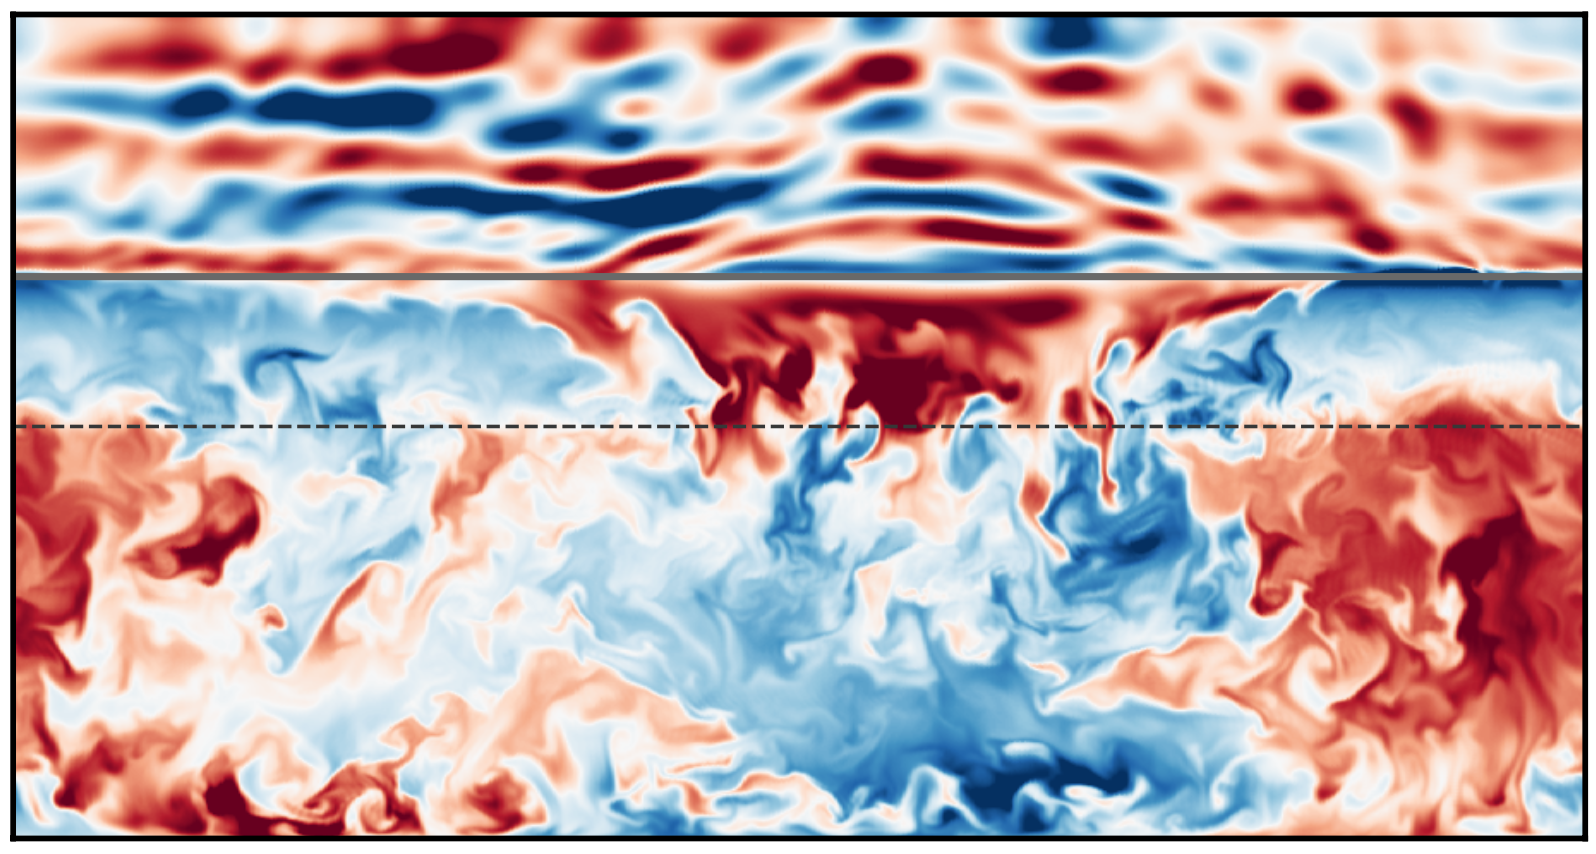
\includegraphics[width=\textwidth]{penconv.png}
%         \caption{Penetrative Convection sim \citep{anders_etal_2022a}}
%         \label{fig:penconv}
%     \end{subfigure}
%     \hfill
%     \begin{subfigure}[b]{0.3\textwidth}
%         \centering
%         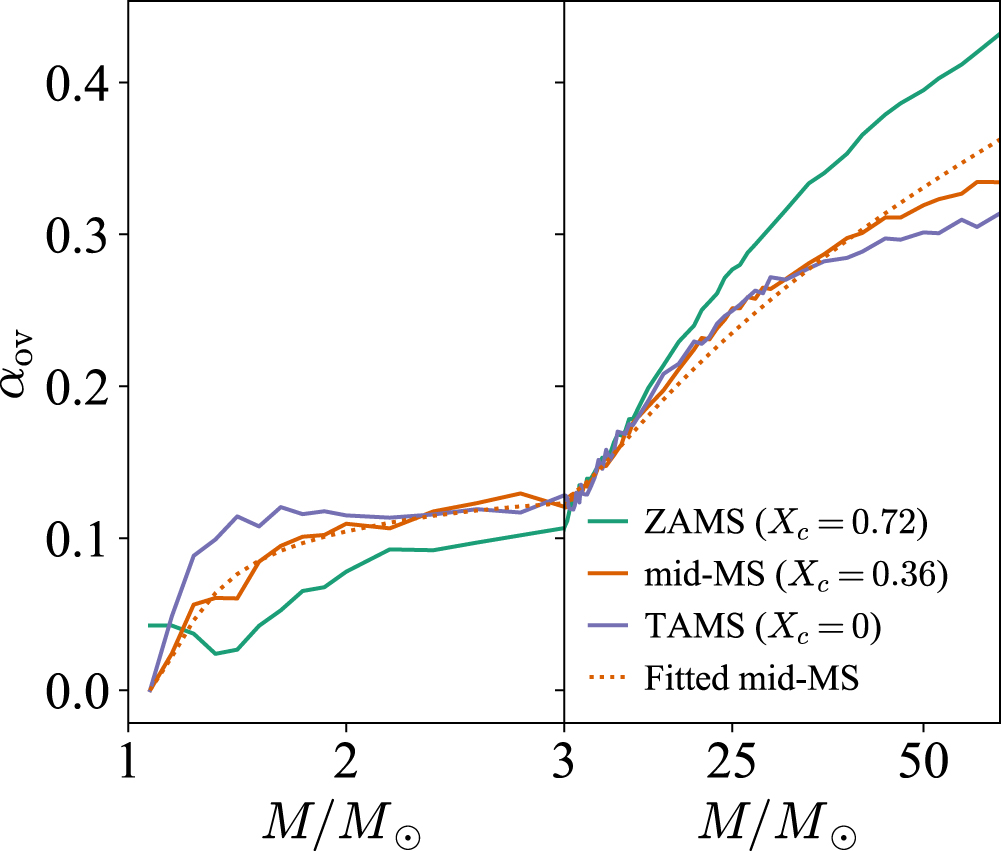
\includegraphics[width=\textwidth]{jermyn2022.jpeg}
%         \caption{Penetrative Convection in stars \citep{jermyn_etal_2022_penconv}}
%         \label{fig:penconv_stars}
%     \end{subfigure}
%     \hfill
%     \begin{subfigure}[b]{0.3\textwidth}
%         \centering
%         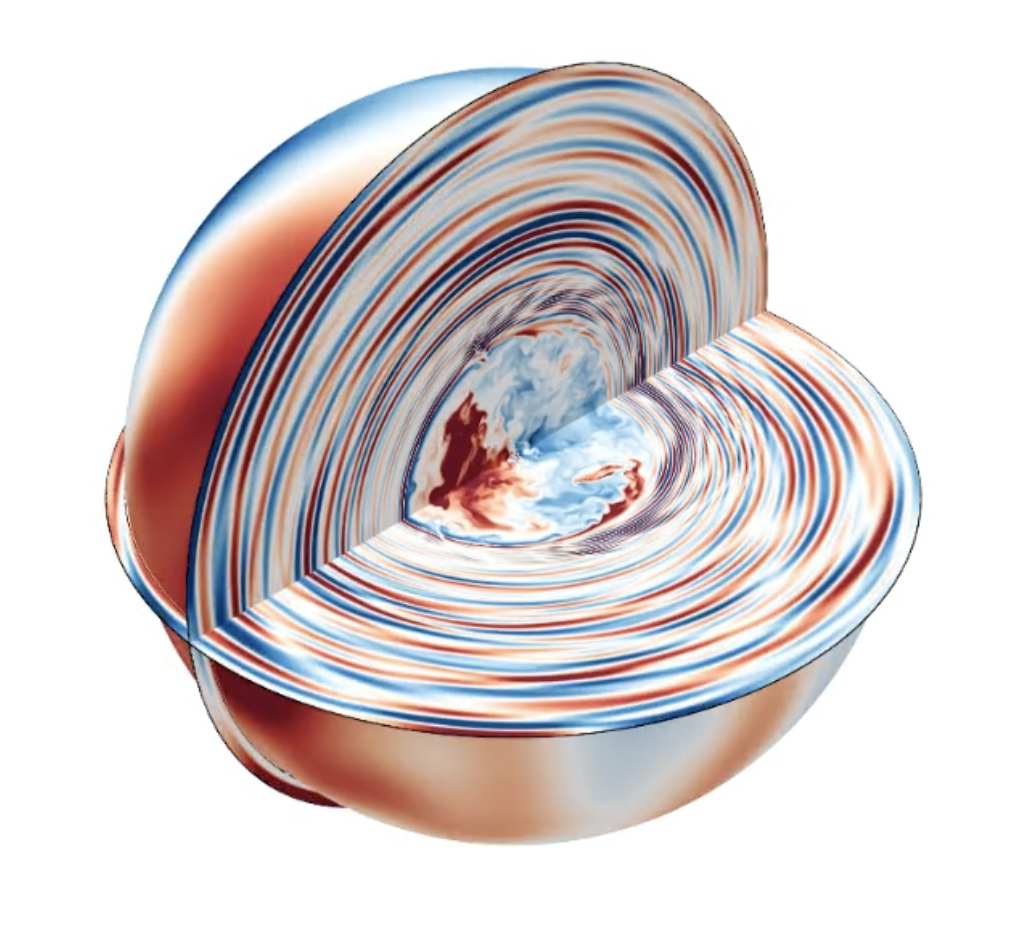
\includegraphics[width=\textwidth]{dedalus_massive_star.png}
%         \caption{Dedalus 40 $M_{\odot}$ sim}
%         \label{fig:dedalus_massive_star}
%     \end{subfigure}
%        \caption{(A) A dedalus simulation exhibiting penetrative convection; note the region between the two horizontal lines where hot upflows (from the bottom CZ) turn cold.
%        (B) Inferred convective mixing in stars using our prescription from \citep{anders_etal_2022a}; note the similar trend to \citep{claret_torres_2019} to the left of the vertical line (same mass range as Fig.~\ref{fig:claret_torres}) and the increase to higher masses to the right side of the line.
%        (C) A Dedalus simulation of core convection in a $40 M_{\odot}$ star run using my preliminary module which I propose to use to explore core convection in this proposal.}
%        \label{fig:intro}
%\end{figure}
%

State-of-the-art simulations also demonstrate that convection prefers larger cores than models predict.
Many simulations have shown rapid turbulent entrainment at convective boundaries in massive and evolved stars (cites), but these simulations are never run for long enough to reach a statistically stationary state.
What's worse, when the entrainment law calibrated to these simulations is put directly into stellar structure models, studies find that the convective core consumes the whole star (cites), which is clearly unphysical.
Convection zones should clearly saturate at some size which is larger than the size given by e.g., the Schwarzschild criterion in standard models.
I recently performed simulations which demonstrated that energetically equilibrated convection zones can expand well beyond the Schwarzschild boundary, and also found a constraint upon the expansion of that convection zone (see Fig.~\ref{fig:penconv}), (cite).
When this constraint is applied in postprocessing to stellar models, we find that this constraint produces mixing of the stellar core which produces similar trends to observations (see Fig.~\ref{fig:penconv_stars}), (cite).
However, this constraint was calibrated in a 3D Cartesian domain, and in the incompressible approximation.

Stellar core convection is traditionally very difficult to simulate.
Many codes include a ``cutout'' near $r = 0$ and so do not truly evolve the full convective core, which may produce unphysical dynamics (cites).
Furthermore, core convection occurs at very low mach numbers (cite atlas, give typical values); frequently-used methods to simulate these low-mach flows include using the anelastic approximation (cites), which does not perform well when regions beyond the convection zone are mixed, or boosting of the luminosity, which may lead to unphysically large overshoot zones (cites).

To address these modeling deficiencies, I will create simulations of the cores of massive stars using the \emph{Dedalus} \citep{burns_etal_2020} code.
These simulations will differ from past simulations of massive stars, because they will include the full ``ball'' geometry of the convective core, they will employ the fully compressible equations without any luminosity boosting, and they will be relaxed into thermal equilibrium; an example of one of these new state-of-the-art simulations is shown in Fig.~\ref{fig:dedalus_massive_star}.
\emph{Dedalus} was recently updated with the state-of-the-art ability to simulate flows that pass through the coordinate singularity at $r = 0$ in spherical coordinates \citep{vasil_etal_2019,lecoanet_etal_2019}; most prior codes used a spherical shell geometry with a small interior ``cutout'' of the core.
We have successfully simulated very low Mach number flows without timestepping restrictions in Dedalus by employing implicit-explicit (IMEX) timestepping techniques; we implicitly step the stiff linear sound waves while explicitly timestepping the nonlinear advective terms, which allows us to accurate take timesteps which follow the convection rather than the fast waves.
Regarding thermal equilibration, my previous CBM studies \citep{anders_etal_2022a,anders_etal_2022b} demonstrated that the structure of boundary mixing regions can take thousands of convective overturn times to saturate.
Fortunately, I have developed methods of ``accelerated evolution'' \citep{anders_etal_2018}; these techniques allow me to achieve thermally equilibrated solutions while saving up to an order of magnitude in computational resources.

TODO: Emphasize in the previosu paragraph that I will publish the code used to create these simulations and design it with ease-of-use for the community in mind.

TODO: Talk about the fact that core convection is also always at low Rossby / is rotationally constrained.

\emph{\underline{Task 1:}} %My previous work \citep{anders_etal_2022a} demonstrated that convective penetration is a process that can be observed in thermally equilibrated, nonlinear convective simulations.
I will study convective penetration \citep[Fig \ref{fig:penconv}, left,][]{anders_etal_2022a}, in fully compressible simulations whose background stratifications are based upon MESA models of massive stars (as in Fig.~\ref{fig:dedalus_massive_star}, middle).
In this first task, I will focus on simulations of non-rotating stars spanning the mass range $M_* = 1.1-40 M_{\odot}$.
I will in particular study the low-mass range from $1.1-3 M_{\odot}$, where observed ``extra mixing'' is a strong function of stellar mass \citep[][Fig.~\ref{fig:claret_torres} and Fig.~\ref{fig:penconv_stars}]{claret_torres_2019}, and compare these simulations to these observations of eclipsing binaries.

\emph{\underline{Task 2:}} I will include rotation into my models to understand how the stellar rotation rate affects convective boundary mixing.
Rotation is theorized to reduce the extent of convective boundary mixing \citep{augustson_mathis_2019}.
In our current theory of CBM via convective penetration \citep{anders_etal_2022a} the mixing region's size depends on the dissipation in the convection zone.
Rotation effectively organizes flows into rotation-aligned vortices with high dissipation rates (cite), so this logically follows, but the degree to which the effect operates must be calibrated.

\textbf{\underline{\emph{Deliverable:}} The first 3D simulations of core convection in massive stars that include the coordinate singularity at $\boldsymbol{r = 0}$, reach thermal equilibrium, and span the main sequence.}
These models will be used to create a 1D implementation of convective boundary mixing informed by realistic simulations in the proper geometry, significantly improving the limited model we presented in \citep{anders_etal_2022a}.
I will also publish an open-source, fully compressible \emph{Dedalus} module, so the community will have straightforward access to a tool to use for studying dynamics in massive stars.

\section{Focus II: Optically thick, low-efficiency Iron-Bump Convection.}
TODO: Add a figure here?

In addition to vigorous core convection, it is now accepted that massive stars have opacity-driven convective shells in their envelopes \citep{cantiello_etal_2009}.
For stars with masses $\gtrsim 8 M_{\odot}$, an ``Iron-Bump Convection Zone'' (FeCZ) appears as a result of the opacity of iron.
These convection zones approach the Eddington luminosity limit, are very thin, exhibit high-mach number, turbulent flows, and are very radiation-dominated \citep{jermyn_etal_2022_atlas}.
However, unlike the convection zones at the surface of lower-mass stars (e.g., the Sun), these convection zones generally appear at high optical depths \citep[fig 59 of][]{jermyn_etal_2022_atlas}.
This is an exotic regime of convection which has not been studied in detail, but the presence of these convection zones influences the stellar structure and evolution appreciably (cites).

In stellar models, the presence of the near-Eddington FeCZs under traditional MLT convective approximation lead to odd stellar model behavior.
These zones often develop density and gass pressure inversions (cite) which inflate the star and must be handled in ad-hoc rather than physical manners \citep{kohler_etal_2015}.
The stellar inflation accompanying these zones reduces the effective surface temperature (cite) which modifies the efficiency of winds launched from the stellar surface, affecting the mass loss achieved by these stars and the subsequent stellar evolution \citep{smith_2014} (cite more?).

Numerical simulations of these convection zones are extremely limited.
A few simulations of FeCZs for 40 and 80 $M_{\odot}$ stars were performed \citep{jiang_etal_2015} and studied in detail \citep{schultz_etal_2020}.
They found extremely interesting dynamics: the envelope about these zones is extremely dynamic, and the high radiative efficiency in these zones lead to dynamics very distinct from e.g., core convection (put in a figure here, talk about it).
However, of particular interest, the high-Mach number convection supports a large amount of dynamic pressure.
Convection mixes the temperature gradient to $\nabla \rightarrow \nabla_{\rm ad} = (d\ln P/ d\ln T)_{\rm ad}$, but the presence of a large dynamical pressure component $P_{\rm dyn}$ modifies the adiabatic gradient $\nabla_{\rm ad}$ and as a result modifies the achieved stellar structure.
Unfortunately the full radiative hydrodynamic simulations in which this was observed are extremely expensive, so it is difficult to understand how this behavior emerges across the HR diagram as a function of stellar mass and stellar age.

Fortunately, the FeCZ generally occurs in a very optically thick regime ($\tau \sim 10^{1-4}$) where the radiative diffusion approximation is valid \citep{jermyn_etal_2022_atlas}.
As a result, it is possible to study these simulations with much less expensive simulations that do not solve the full equations of radiative transfer but which do still include the iron opacity peak and high mach number flows.
Furthermore, since these convection zones are generally very thin (aspect ratios $r / \delta r \sim 10^{1-3}$), modeling these zones in a plane-parallel Cartesian domain is a good approximation.
I will use \emph{Dedalus} to build on the high-Mach number, fully compressible simulations that I studied in Ref.~\citep{anders_brown_2017} by including iron bump opacity effects.
I will study a span of simulations varying stellar mass from $8-60 M_{\odot}$ and from the ZAMS to the TAMS to understand the turbulent pressure component that arises from these simulations in order to improve the stratification in stellar models without needing ad-hoc solutions.

Furthermore, there is a current debate about whether ``red noise'' or ``stochastic low-frequency variability,'' (SLFV) which is a ubiquitous signal observed in massive stars \citep{bowman_etal_2019}, is the signal of gravity waves generated in the convective core or a result of turbulent motions generated by surface convection zones.
A number of simulations of core generated gravity waves have been performed (cites), but these simulations do not include the FeCZ and so it is impossible to tell how this zone would affect these waves.
An examination of turbulent motions generated by the FeCZ suggest that they could be coincident with SLFV \citep{schultz_etal_2022}, but further studies are needed.
After studying how the FeCZ generates a turbulent pressure to alter the stellar stratification, I will study how the FeCZ modifies the signal of gravity waves generated by core convection.
I will include the stable radiative zone surrounding the FeCZ in my simulations and force a spectrum of gravity waves at the bottom boundary, then measure how these waves interact with and are modified by the turbulent convection in the FeCZ.

\emph{\underline{Task 3:}} I will study iron bump convection in Cartesian, optically thick models which span from $8-60 M_{\odot}$ and which include ZAMS models, mid-MS models, and TAMS models.
I will measure how the turbulent pressure compares to the background pressure, and parameterize this for inclusion in 1D stellar evolution models like MESA.
I will work with experts in the MESA community to include this parameterization into stellar evolution models, then I will evolve a new suite of state-of-the-art stellar evolution models which include these modified pressure effects to understand how this affects the stellar radius, effective temperature, and other observables of these stars.

\emph{\underline{Task 4:}} I will study how FeCZs modify gravity wave signals from core convection.
Core-generated gravity waves are one of the most promising tools for putting constraints on the interior structure of massive stars (cites).
These simulations will put the first constraints on whether or not gravity waves can pass through the FeCZ to be observable at the stellar surface.
The results of these simulations will help determine whether observers should look towards lower-metallicity, lower-mass stars where there are no opacity-driven convection zones for wave signals \citep{jermyn_etal_2022_window}.

\textbf{\underline{\emph{Deliverable:}} The first 3D simulations of iron-bump convection spanning the HR diagram.}
These simulations will be used to create a 1D implementation of turbulent pressure support generated by the FeCZ, which will improve stellar structure and evolution models of massive stars.
These simulations will then be used to create the first experimental test of whether core generated gravity waves can pass through the turbulent motions in the FeCZ to be observed at the surface.
As with tasks 1-2, the \emph{Dedalus} simulation tools used to create these FeCZ simulations will be published and made widely accessible.



\sct{Focus III: Convective Blueshift}
%\textbf{Matt: Task 4 -- say explicitly that I'm envisioning local Cartesian. Comment that I intend to work broadly in parallel on tasks 1-3 and tasks 4-5. Include paper writing in the timeline. We will also participate in the public outreach and public engagement stuff at Exeter.}
An Earth-like planet around a Sun-like star produces a radial velocity (RV) signal on the order of 10 cm/s.
Extreme Precision RV (EPRV) instruments are now sensitive enough to observe signals below this threshold, but stellar surface convection produces RV signals much larger than 10 cm/s \citep{crass_etal_2021}.
``Convective Blueshift" (CBS) is a net blueshifting of spectral line wings resulting from the convection granulation pattern (warm upflows cover more surface area than cold downflows).
CBS measurements were recently obtained for hundreds of stars \citep{liebing_etal_2021}; a tight cubic relationship is found between the effective temperature and CBS, which may result from the changing size of convective granules. %careful about "robust"
In order to robustly remove CBS from EPRV signals, empirical fits must be tested and validated against theory and nonlinear magnetoconvection simulations. 

Convection at the Sun's surface has been studied in exquisite detail in Cartesian simulations which include full radiative transfer (RT) treatments \citep[e.g.,][]{rempel2020, danilovic_etal_2022}.
Unfortunately this full RT treatment makes these simulations costly, so studying CBS across the lower main sequence is not feasible.
I will develop magnetoconvection simulations with reduced models of RT.
Using a computationally efficient but still realistic RT treatment, I will create a simulation suite spanning the lower main sequence and create synthesized observables to compare with existing CBS datasets.

The University of Exeter is deeply involved in the Terra Hunting Experiment (Profs.~Naylor \& Baraffe and Dr.~Haywood), which will survey G and K-type stars with the HARPS III high-resolution spectrograph at the Isaac Newton telescope every night for 10 or more years.
This survey will provide extremely precise data on the activity and surface dynamics of the stars, and should start in 2023-2024.
Data from this survey will be ready to use to validate my simulations when I arrive at Exeter.

\underline{\emph{Task 4:}} I will create fully compressible magnetoconvection simulations in \emph{Dedalus} in a local, Cartesian model of a stellar surface using three different levels of approximation for radiative transfer.
I will implement convection under the Eddington tensor approximation \citep[previously tested in \emph{Dedalus} in ref.][sct.~XI.G]{burns_etal_2020}, under the approximation of a grey atmosphere with a ``realistic'' radiative diffusivity \citep{barekat_brandenburg_2014}, and under a simplified diffusion approximation with an idealized radiative diffusivity and an imposed surface cooling.
I will test how properties such as the size and flow speed of convective granules vary across these approximations.
I will choose the simplest approximation with the highest fidelity to the Eddington tensor solution to use in future CBS simulations.

\underline{\emph{Task 5:}} I will create a suite of local simulations of surface convection spanning the lower main sequence.
I will synthesize observables of CBS and compare these to observations \citep{liebing_etal_2021}, including those which will be obtained at Exeter from HARPS III.
I will work alongside members of the Terra Hunting Experiment to refine CBS prescriptions based on these results.

\textbf{\underline{\emph{Deliverable:}} The first simulated constraint from 3D MHD simulations on convective blueshift spanning the lower main sequence.}
%I will also synthesize CBS observables from these simulations and collaborate with the Terra Hunting Experiment to improve CBS models.


\paragraph*{Research and Outreach}
I love teaching and am excited to teach any of the undergraduate mathematics or physics courses offered by the School. 
As for graduate education, my research background has best prepared me to lead the Theoretical Physics ``Computational Research Skills in Physics'' MRes module or to mentor a research component under the ``Astrophysics and Geophysics'' theme.
I currently co-mentor five graduate students, and have co-mentored undergraduate students in the past; I look forward to starting a vibrant research group where PhD, MRes, and undergraduate students all feel welcome, and where individuals whose identities are underrepresented in mathematics, physics and astrophysics can build confidence and identities as people in STEM.
When I was a graduate student at the University of Colorado, I created and iterated upon the first rubric used in the graduate admissions process to make it more equitable and I would love to work on similar processes at Newcastle.
As a postdoctoral fellow at CIERA, I chaired a public outreach committee for a year and have been actively involved in organizing a climate survey for the 2022-2023 academic year.
I enjoy working to make my department a more fair, equitable, and just place, and I will bring this dedication and drive with me to Newcastle.

{\scriptsize
\bibliography{biblio}
}
\end{document}
